%%%%%%%%%%%%%%%%%%%%%%%%%%%%%%%%%%%%%%
%%%%%%%%%%%%%%%%%%%%%%%%%%%%%%%%%%%%%%
% Do not edit the TeX file your work
% will be overwritten.  Edit the RnW
% file instead.
%%%%%%%%%%%%%%%%%%%%%%%%%%%%%%%%%%%%%%
%%%%%%%%%%%%%%%%%%%%%%%%%%%%%%%%%%%%%%



%


\begin{knitrout}
\definecolor{shadecolor}{rgb}{0.969, 0.969, 0.969}\color{fgcolor}\begin{figure}[!h]

{\centering 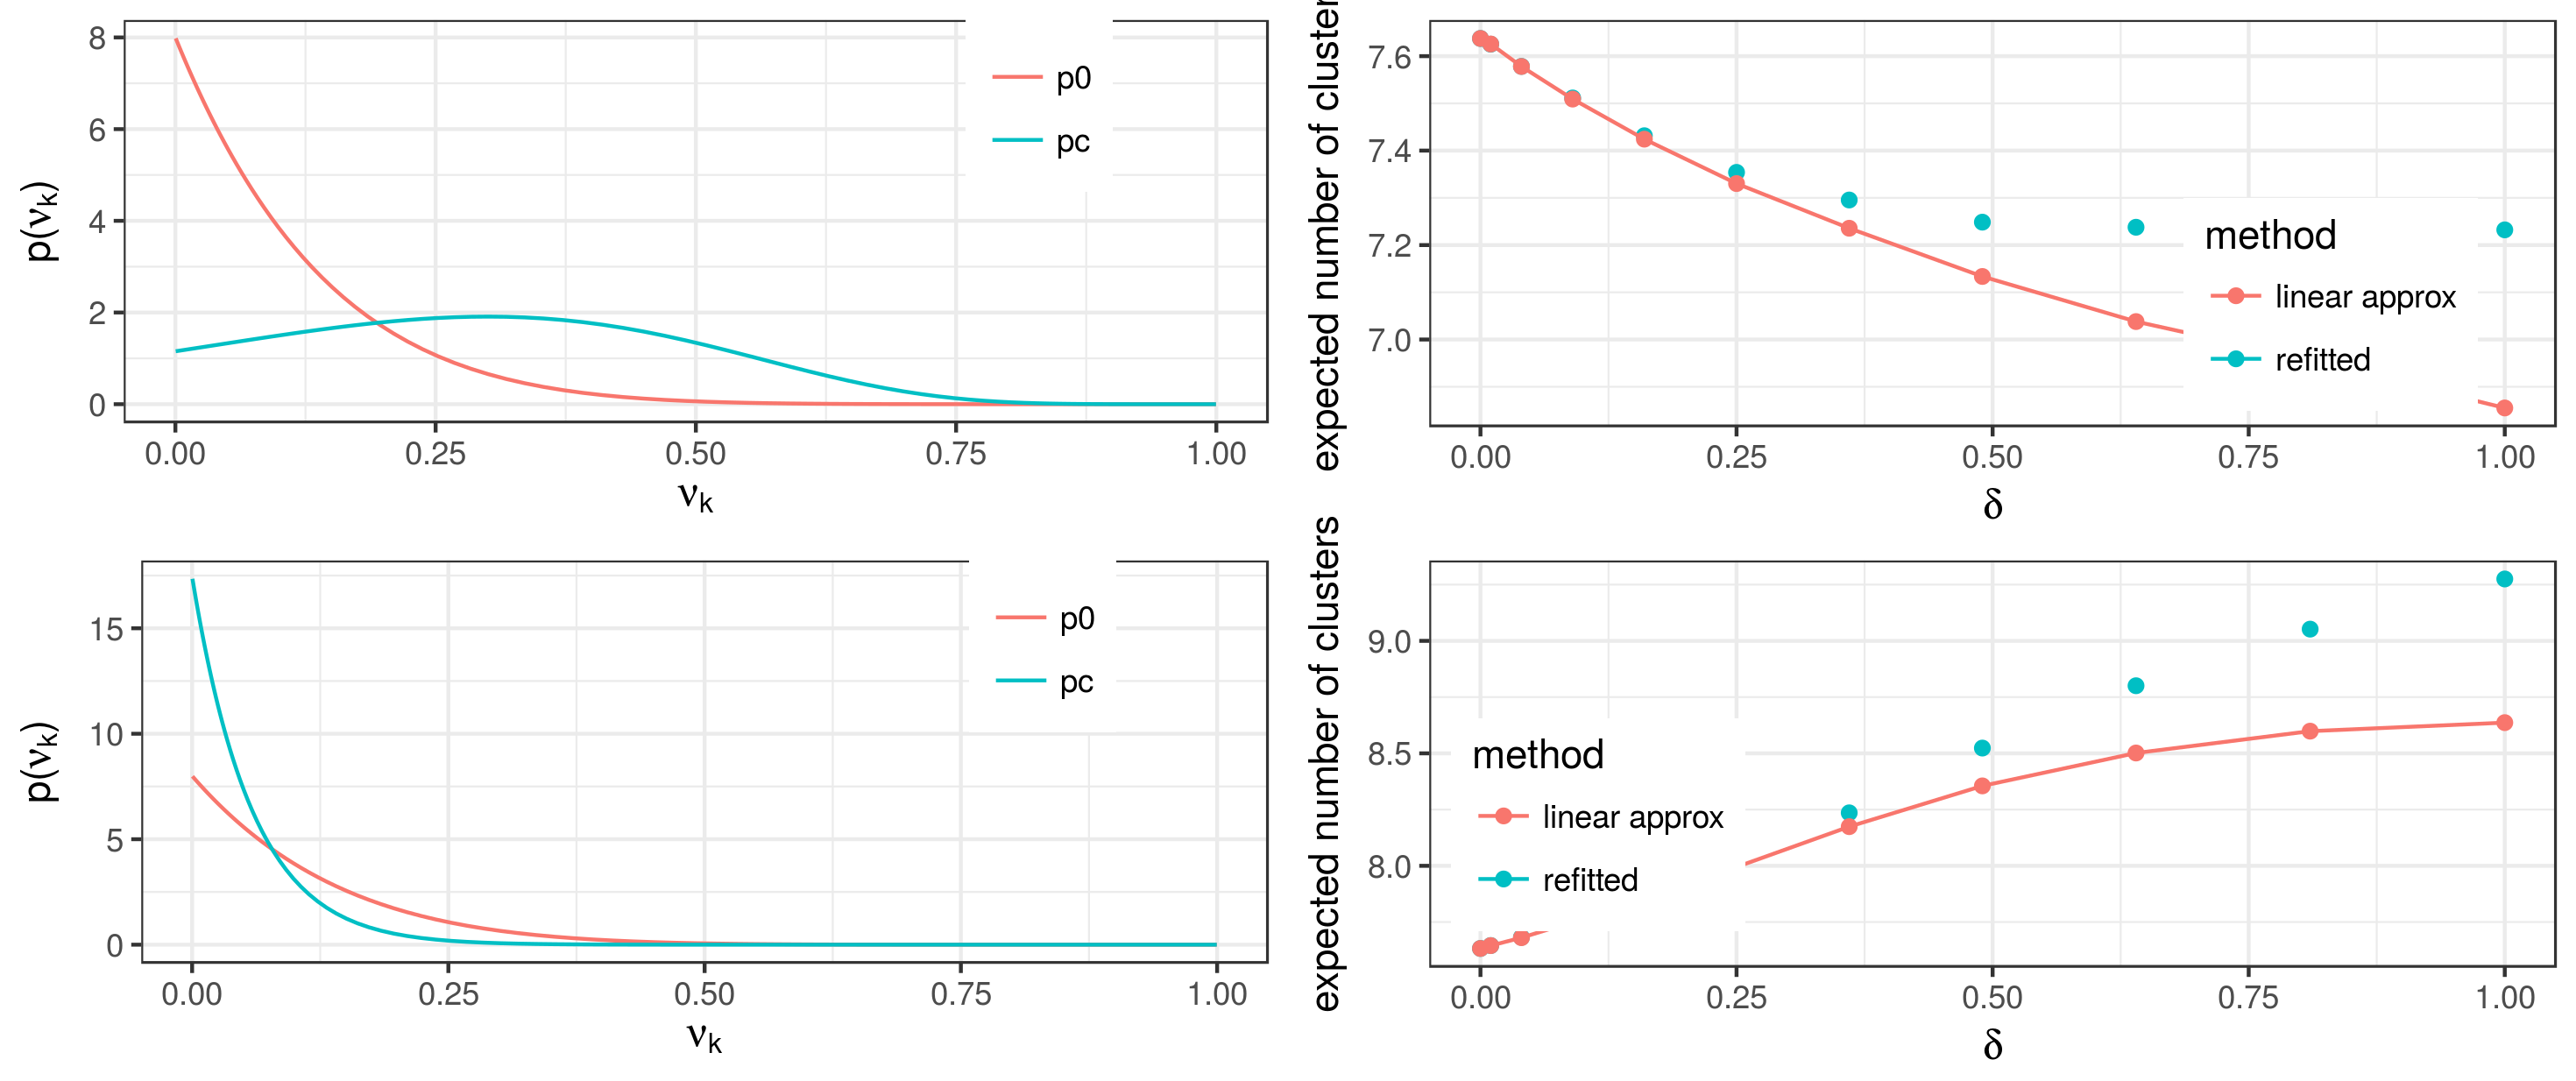
\includegraphics[width=0.98\linewidth,height=0.294\linewidth]{figure/functional_sens_plot-1} 

}

\caption{\label{fig:func_sens_e_num_clusters}
Left column: the original prior $p_{0}$ in orange,
the perturbed prior $p_c$ in green. Right: linearly approximated vs.
re-fitted expected number of clusters after the perturbation.  }\label{fig:functional_sens_plot}
\end{figure}


\end{knitrout}
%
In \prettyref{fig:functional_sens_plot}, we show results for the functional
perturbation $\phi(\nu_k) = 1 - e^{\nu_k}$.
We find that the linear approximation in this case was able to capture the
direction of the perturbation, (the expected number of clusters increased under
the first perturbation, decreased under the second), although as $\delta
\rightarrow 1$ the quality of the approximation degraded.
